
\section{Measurements}\label{sec:measurements}

\subsection{Measurement Setup}

Development nodes: 301, 520


\clearpage
\subsection{Video Preparation}

Table~\ref{tab:videos} lists the videos we have prepared for \ac{DASH}. Videos with a duration longer than $5$ minutes were selected.

\begin{table}[h!]
\centering
\caption{Selected videos.}
\begin{tabular}{|c|c|c|c|}
\hline
\textbf{Internal ID} & \textbf{Category} & \textbf{YTID} & \textbf{Description / Title} \\
\hline
0 & Animation & & BigBuckBunny\\
\hline
1 & Sport & D8YQn7o\_AyA & Deutschland vs. Italien Elfmeterschie\ss en\\
\hline
2 & Documentary & 6v2L2UGZJAM & Planet Earth: Amazing nature scenery\\
\hline
3 & Animation & Y-rmzh0PI3c & Cosmos Laundromat - First Cycle\\
\hline
4 & Entertainment (Talkshow) & N2sCbtodGMI & DIY Musikinstrumente ? Hazel Brugger\\
\hline
5& ... & & \\
\hline
\end{tabular}
\label{tab:videos}
\end{table}

\textbf{Video1: D8YQn7o\_AyA}
%Video 1: Deutschland vs Italien Elfmeterschie�en, ID: D8YQn7o_AyA, Category: Sport
\begin{itemize}
\item Has fragments: 133, 134, 135, 136, 137, 160, 264, 266, 298, 299
\item No fragments (dropped): 18, 22
\item Alignment problem, check GOP (dropped): 298, 299
\item Final: 8 representations (133, 134, 135, 136, 137, 160, 264, 266)
\end{itemize}

\begin{figure} [h!]
\caption{Video 1.}
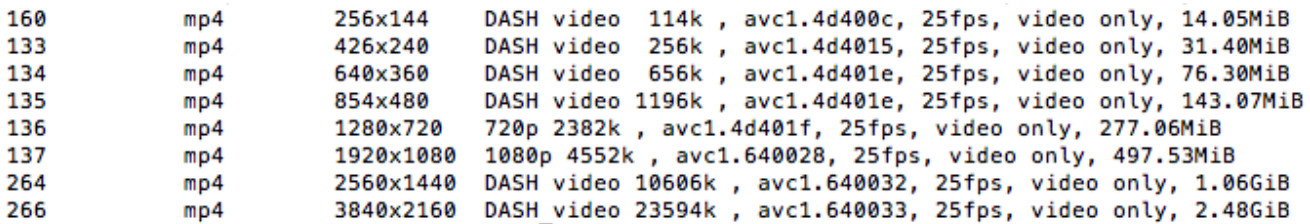
\includegraphics[width=\textwidth]{graphics/video1}
\label{fig:video1}
\end{figure}

\textbf{Video2: 6v2L2UGZJAM}
%Video 2: Planet Earth: Amazing nature scenery, ID: 6v2L2UGZJAM, Categorie: Documentary
\begin{itemize}
\item Has fragments: 133, 134, 135, 136, 137, 160, 212, 213, 214, 215, 216, 217
\item No fragments (dropped): 18, 22
\item Alignment problem, check GOP (dropped):
\end{itemize}




\clearpage
\subsection{Measurement Campaigns}

Measurement campaign checklist:
\begin{itemize}
\item AStream server up
\item All video \acp{MPD} on AStream server
\item Config file control
\item Trial on development node
\end{itemize}

Table~\ref{tab:measurements} lists the measurement campaigns.

\begin{table}[h!]
\centering
\caption{Measurement campaigns.}
\begin{tabular}{|c|c|c|c|}
\hline
\textbf{Date} & \textbf{Number of Batches} & \textbf{Number of Nodes} & \textbf{Other} \\
\hline
&&&\\
\hline
&&&\\
\hline
&&&\\
\hline
\end{tabular}
\label{tab:measurements}
\end{table}

